\documentclass[1p]{elsarticle_modified}
%\bibliographystyle{elsarticle-num}

%\usepackage[colorlinks]{hyperref}
%\usepackage{abbrmath_seonhwa} %\Abb, \Ascr, \Acal ,\Abf, \Afrak
\usepackage{amsfonts}
\usepackage{amssymb}
\usepackage{amsmath}
\usepackage{amsthm}
\usepackage{scalefnt}
\usepackage{amsbsy}
\usepackage{kotex}
\usepackage{caption}
\usepackage{subfig}
\usepackage{color}
\usepackage{graphicx}
\usepackage{xcolor} %% white, black, red, green, blue, cyan, magenta, yellow
\usepackage{float}
\usepackage{setspace}
\usepackage{hyperref}

\usepackage{tikz}
\usetikzlibrary{arrows}

\usepackage{multirow}
\usepackage{array} % fixed length table
\usepackage{hhline}

%%%%%%%%%%%%%%%%%%%%%
\makeatletter
\renewcommand*\env@matrix[1][\arraystretch]{%
	\edef\arraystretch{#1}%
	\hskip -\arraycolsep
	\let\@ifnextchar\new@ifnextchar
	\array{*\c@MaxMatrixCols c}}
\makeatother %https://tex.stackexchange.com/questions/14071/how-can-i-increase-the-line-spacing-in-a-matrix
%%%%%%%%%%%%%%%

\usepackage[normalem]{ulem}

\newcommand{\msout}[1]{\ifmmode\text{\sout{\ensuremath{#1}}}\else\sout{#1}\fi}
%SOURCE: \msout is \stkout macro in https://tex.stackexchange.com/questions/20609/strikeout-in-math-mode

\newcommand{\cancel}[1]{
	\ifmmode
	{\color{red}\msout{#1}}
	\else
	{\color{red}\sout{#1}}
	\fi
}

\newcommand{\add}[1]{
	{\color{blue}\uwave{#1}}
}

\newcommand{\replace}[2]{
	\ifmmode
	{\color{red}\msout{#1}}{\color{blue}\uwave{#2}}
	\else
	{\color{red}\sout{#1}}{\color{blue}\uwave{#2}}
	\fi
}

\newcommand{\Sol}{\mathcal{S}} %segment
\newcommand{\D}{D} %diagram
\newcommand{\A}{\mathcal{A}} %arc


%%%%%%%%%%%%%%%%%%%%%%%%%%%%%5 test

\def\sl{\operatorname{\textup{SL}}(2,\Cbb)}
\def\psl{\operatorname{\textup{PSL}}(2,\Cbb)}
\def\quan{\mkern 1mu \triangleright \mkern 1mu}

\theoremstyle{definition}
\newtheorem{thm}{Theorem}[section]
\newtheorem{prop}[thm]{Proposition}
\newtheorem{lem}[thm]{Lemma}
\newtheorem{ques}[thm]{Question}
\newtheorem{cor}[thm]{Corollary}
\newtheorem{defn}[thm]{Definition}
\newtheorem{exam}[thm]{Example}
\newtheorem{rmk}[thm]{Remark}
\newtheorem{alg}[thm]{Algorithm}

\newcommand{\I}{\sqrt{-1}}
\begin{document}

%\begin{frontmatter}
%
%\title{Boundary parabolic representations of knots up to 8 crossings}
%
%%% Group authors per affiliation:
%\author{Yunhi Cho} 
%\address{Department of Mathematics, University of Seoul, Seoul, Korea}
%\ead{yhcho@uos.ac.kr}
%
%
%\author{Seonhwa Kim} %\fnref{s_kim}}
%\address{Center for Geometry and Physics, Institute for Basic Science, Pohang, 37673, Korea}
%\ead{ryeona17@ibs.re.kr}
%
%\author{Hyuk Kim}
%\address{Department of Mathematical Sciences, Seoul National University, Seoul 08826, Korea}
%\ead{hyukkim@snu.ac.kr}
%
%\author{Seokbeom Yoon}
%\address{Department of Mathematical Sciences, Seoul National University, Seoul, 08826,  Korea}
%\ead{sbyoon15@snu.ac.kr}
%
%\begin{abstract}
%We find all boundary parabolic representation of knots up to 8 crossings.
%
%\end{abstract}
%\begin{keyword}
%    \MSC[2010] 57M25 
%\end{keyword}
%
%\end{frontmatter}

%\linenumbers
%\tableofcontents
%
\newcommand\colored[1]{\textcolor{white}{\rule[-0.35ex]{0.8em}{1.4ex}}\kern-0.8em\color{red} #1}%
%\newcommand\colored[1]{\textcolor{white}{ #1}\kern-2.17ex	\textcolor{white}{ #1}\kern-1.81ex	\textcolor{white}{ #1}\kern-2.15ex\color{red}#1	}

{\Large $\underline{12n_{0122}~(K12n_{0122})}$}

\setlength{\tabcolsep}{10pt}
\renewcommand{\arraystretch}{1.6}
\vspace{1cm}\begin{tabular}{m{100pt}>{\centering\arraybackslash}m{274pt}}
\multirow{5}{120pt}{
	\centering
	\includegraphics[width=112pt]{../../../GIT/diagram.site/Diagrams/png/2211_12n_0122.png}\\
\ \ \ A knot diagram\footnotemark}&
\allowdisplaybreaks
\textbf{Linearized knot diagam} \\
\cline{2-2}
 &
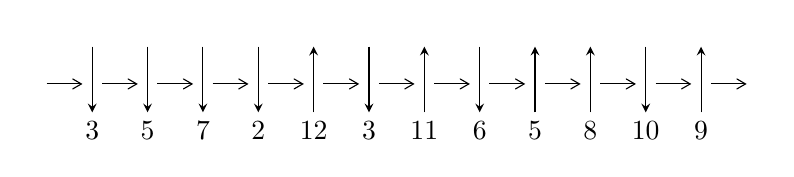
\begin{tikzpicture}[x=20pt, y=17pt]
	% nodes
	\node (C0) at (0, 0) {};
	\node (C1) at (1, 0) {};
	\node (C1U) at (1, +1) {};
	\node (C1D) at (1, -1) {3};

	\node (C2) at (2, 0) {};
	\node (C2U) at (2, +1) {};
	\node (C2D) at (2, -1) {5};

	\node (C3) at (3, 0) {};
	\node (C3U) at (3, +1) {};
	\node (C3D) at (3, -1) {7};

	\node (C4) at (4, 0) {};
	\node (C4U) at (4, +1) {};
	\node (C4D) at (4, -1) {2};

	\node (C5) at (5, 0) {};
	\node (C5U) at (5, +1) {};
	\node (C5D) at (5, -1) {12};

	\node (C6) at (6, 0) {};
	\node (C6U) at (6, +1) {};
	\node (C6D) at (6, -1) {3};

	\node (C7) at (7, 0) {};
	\node (C7U) at (7, +1) {};
	\node (C7D) at (7, -1) {11};

	\node (C8) at (8, 0) {};
	\node (C8U) at (8, +1) {};
	\node (C8D) at (8, -1) {6};

	\node (C9) at (9, 0) {};
	\node (C9U) at (9, +1) {};
	\node (C9D) at (9, -1) {5};

	\node (C10) at (10, 0) {};
	\node (C10U) at (10, +1) {};
	\node (C10D) at (10, -1) {8};

	\node (C11) at (11, 0) {};
	\node (C11U) at (11, +1) {};
	\node (C11D) at (11, -1) {10};

	\node (C12) at (12, 0) {};
	\node (C12U) at (12, +1) {};
	\node (C12D) at (12, -1) {9};
	\node (C13) at (13, 0) {};

	% arrows
	\draw[->,>={angle 60}]
	(C0) edge (C1) (C1) edge (C2) (C2) edge (C3) (C3) edge (C4) (C4) edge (C5) (C5) edge (C6) (C6) edge (C7) (C7) edge (C8) (C8) edge (C9) (C9) edge (C10) (C10) edge (C11) (C11) edge (C12) (C12) edge (C13) ;	\draw[->,>=stealth]
	(C1U) edge (C1D) (C2U) edge (C2D) (C3U) edge (C3D) (C4U) edge (C4D) (C5D) edge (C5U) (C6U) edge (C6D) (C7D) edge (C7U) (C8U) edge (C8D) (C9D) edge (C9U) (C10D) edge (C10U) (C11U) edge (C11D) (C12D) edge (C12U) ;
	\end{tikzpicture} \\
\hhline{~~} \\& 
\textbf{Solving Sequence} \\ \cline{2-2} 
 &
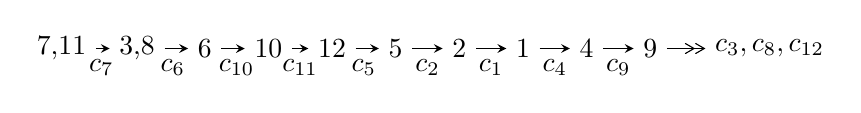
\begin{tikzpicture}[x=23pt, y=7pt]
	% node
	\node (A0) at (-1/8, 0) {7,11};
	\node (A1) at (17/16, 0) {3,8};
	\node (A2) at (17/8, 0) {6};
	\node (A3) at (25/8, 0) {10};
	\node (A4) at (33/8, 0) {12};
	\node (A5) at (41/8, 0) {5};
	\node (A6) at (49/8, 0) {2};
	\node (A7) at (57/8, 0) {1};
	\node (A8) at (65/8, 0) {4};
	\node (A9) at (73/8, 0) {9};
	\node (C1) at (1/2, -1) {$c_{7}$};
	\node (C2) at (13/8, -1) {$c_{6}$};
	\node (C3) at (21/8, -1) {$c_{10}$};
	\node (C4) at (29/8, -1) {$c_{11}$};
	\node (C5) at (37/8, -1) {$c_{5}$};
	\node (C6) at (45/8, -1) {$c_{2}$};
	\node (C7) at (53/8, -1) {$c_{1}$};
	\node (C8) at (61/8, -1) {$c_{4}$};
	\node (C9) at (69/8, -1) {$c_{9}$};
	\node (A10) at (11, 0) {$c_{3},c_{8},c_{12}$};

	% edge
	\draw[->,>=stealth]	
	(A0) edge (A1) (A1) edge (A2) (A2) edge (A3) (A3) edge (A4) (A4) edge (A5) (A5) edge (A6) (A6) edge (A7) (A7) edge (A8) (A8) edge (A9) ;
	\draw[->>,>={angle 60}]	
	(A9) edge (A10);
\end{tikzpicture} \\ 

\end{tabular} \\

\footnotetext{
The image of knot diagram is generated by the software ``\textbf{Draw programme}" developed by Andrew Bartholomew(\url{http://www.layer8.co.uk/maths/draw/index.htm\#Running-draw}), where we modified some parts for our purpose(\url{https://github.com/CATsTAILs/LinksPainter}).
}\phantom \\ \newline 
\centering \textbf{Ideals for irreducible components\footnotemark of $X_{\text{par}}$} 
 
\begin{align*}
I^u_{1}&=\langle 
-5.51787\times10^{81} u^{67}+2.11041\times10^{82} u^{66}+\cdots+3.86959\times10^{83} b+2.32790\times10^{83},\\
\phantom{I^u_{1}}&\phantom{= \langle  }2.89477\times10^{83} u^{67}-1.45377\times10^{84} u^{66}+\cdots+3.86959\times10^{83} a+1.55319\times10^{85},\;u^{68}-5 u^{67}+\cdots+61 u+1\rangle \\
I^u_{2}&=\langle 
b,\;- u^8+2 u^7-3 u^6+2 u^5-3 u^4+2 u^3-2 u^2+a-1,\;u^9- u^8+2 u^7- u^6+3 u^5- u^4+2 u^3+u+1\rangle \\
I^u_{3}&=\langle 
-120 a^2 u-76 a^2-865 a u+691 b-663 a+177 u+43,\;a^3- a^2 u+7 a^2-4 a u-3 a-5 u-12,\\
\phantom{I^u_{3}}&\phantom{= \langle  }u^2+u+1\rangle \\
\\
\end{align*}
\raggedright * 3 irreducible components of $\dim_{\mathbb{C}}=0$, with total 83 representations.\\
\footnotetext{All coefficients of polynomials are rational numbers. But the coefficients are sometimes approximated in decimal forms when there is not enough margin.}
\newpage
\renewcommand{\arraystretch}{1}
\centering \section*{I. $I^u_{1}= \langle -5.52\times10^{81} u^{67}+2.11\times10^{82} u^{66}+\cdots+3.87\times10^{83} b+2.33\times10^{83},\;2.89\times10^{83} u^{67}-1.45\times10^{84} u^{66}+\cdots+3.87\times10^{83} a+1.55\times10^{85},\;u^{68}-5 u^{67}+\cdots+61 u+1 \rangle$}
\flushleft \textbf{(i) Arc colorings}\\
\begin{tabular}{m{7pt} m{180pt} m{7pt} m{180pt} }
\flushright $a_{7}=$&$\begin{pmatrix}1\\0\end{pmatrix}$ \\
\flushright $a_{11}=$&$\begin{pmatrix}0\\u\end{pmatrix}$ \\
\flushright $a_{3}=$&$\begin{pmatrix}-0.748081 u^{67}+3.75690 u^{66}+\cdots+210.979 u-40.1384\\0.0142596 u^{67}-0.0545384 u^{66}+\cdots-3.15431 u-0.601589\end{pmatrix}$ \\
\flushright $a_{8}=$&$\begin{pmatrix}1\\- u^2\end{pmatrix}$ \\
\flushright $a_{6}=$&$\begin{pmatrix}-0.341935 u^{67}+1.84496 u^{66}+\cdots+122.527 u-21.0582\\-0.0113435 u^{67}+0.205218 u^{66}+\cdots+3.86731 u-0.239724\end{pmatrix}$ \\
\flushright $a_{10}=$&$\begin{pmatrix}- u\\u^3+u\end{pmatrix}$ \\
\flushright $a_{12}=$&$\begin{pmatrix}- u^3\\u^5+u^3+u\end{pmatrix}$ \\
\flushright $a_{5}=$&$\begin{pmatrix}-0.338281 u^{67}+1.62581 u^{66}+\cdots+112.042 u-21.2277\\0.0236591 u^{67}-0.0564694 u^{66}+\cdots+3.36495 u-0.255517\end{pmatrix}$ \\
\flushright $a_{2}=$&$\begin{pmatrix}-0.330587 u^{67}+1.67938 u^{66}+\cdots+116.221 u-23.6818\\0.0236591 u^{67}-0.0564694 u^{66}+\cdots+3.36495 u-0.255517\end{pmatrix}$ \\
\flushright $a_{1}=$&$\begin{pmatrix}0.0416035 u^{67}-0.370846 u^{66}+\cdots-11.8634 u+0.807059\\0.0469200 u^{67}-0.282851 u^{66}+\cdots-0.607431 u+0.0154252\end{pmatrix}$ \\
\flushright $a_{4}=$&$\begin{pmatrix}-0.762341 u^{67}+3.81144 u^{66}+\cdots+214.133 u-39.5368\\0.0142596 u^{67}-0.0545384 u^{66}+\cdots-3.15431 u-0.601589\end{pmatrix}$ \\
\flushright $a_{9}=$&$\begin{pmatrix}0.105467 u^{67}-0.401649 u^{66}+\cdots-40.5394 u+7.48605\\-0.151780 u^{67}+0.736790 u^{66}+\cdots+7.94430 u+0.222620\end{pmatrix}$\\&\end{tabular}
\flushleft \textbf{(ii) Obstruction class $= -1$}\\~\\
\flushleft \textbf{(iii) Cusp Shapes $= -0.145860 u^{67}+0.285659 u^{66}+\cdots+33.4674 u-8.97504$}\\~\\
\newpage\renewcommand{\arraystretch}{1}
\flushleft \textbf{(iv) u-Polynomials at the component}\newline \\
\begin{tabular}{m{50pt}|m{274pt}}
Crossings & \hspace{64pt}u-Polynomials at each crossing \\
\hline $$\begin{aligned}c_{1}\end{aligned}$$&$\begin{aligned}
&u^{68}+72 u^{67}+\cdots-116 u+1
\end{aligned}$\\
\hline $$\begin{aligned}c_{2},c_{4}\end{aligned}$$&$\begin{aligned}
&u^{68}-12 u^{67}+\cdots+4 u-1
\end{aligned}$\\
\hline $$\begin{aligned}c_{3},c_{6}\end{aligned}$$&$\begin{aligned}
&u^{68}+3 u^{67}+\cdots+2048 u+512
\end{aligned}$\\
\hline $$\begin{aligned}c_{5}\end{aligned}$$&$\begin{aligned}
&u^{68}+4 u^{67}+\cdots+20 u^2-1
\end{aligned}$\\
\hline $$\begin{aligned}c_{7},c_{10}\end{aligned}$$&$\begin{aligned}
&u^{68}+5 u^{67}+\cdots-61 u+1
\end{aligned}$\\
\hline $$\begin{aligned}c_{8}\end{aligned}$$&$\begin{aligned}
&u^{68}-8 u^{67}+\cdots-679 u+1423
\end{aligned}$\\
\hline $$\begin{aligned}c_{9}\end{aligned}$$&$\begin{aligned}
&u^{68}-4 u^{67}+\cdots-1569175 u-179693
\end{aligned}$\\
\hline $$\begin{aligned}c_{11}\end{aligned}$$&$\begin{aligned}
&u^{68}+33 u^{67}+\cdots-4365 u+1
\end{aligned}$\\
\hline $$\begin{aligned}c_{12}\end{aligned}$$&$\begin{aligned}
&u^{68}+6 u^{67}+\cdots-992 u+64
\end{aligned}$\\
\hline
\end{tabular}\\~\\
\newpage\renewcommand{\arraystretch}{1}
\flushleft \textbf{(v) Riley Polynomials at the component}\newline \\
\begin{tabular}{m{50pt}|m{274pt}}
Crossings & \hspace{64pt}Riley Polynomials at each crossing \\
\hline $$\begin{aligned}c_{1}\end{aligned}$$&$\begin{aligned}
&y^{68}-140 y^{67}+\cdots+13088 y+1
\end{aligned}$\\
\hline $$\begin{aligned}c_{2},c_{4}\end{aligned}$$&$\begin{aligned}
&y^{68}-72 y^{67}+\cdots+116 y+1
\end{aligned}$\\
\hline $$\begin{aligned}c_{3},c_{6}\end{aligned}$$&$\begin{aligned}
&y^{68}-51 y^{67}+\cdots-1048576 y+262144
\end{aligned}$\\
\hline $$\begin{aligned}c_{5}\end{aligned}$$&$\begin{aligned}
&y^{68}-16 y^{67}+\cdots-40 y+1
\end{aligned}$\\
\hline $$\begin{aligned}c_{7},c_{10}\end{aligned}$$&$\begin{aligned}
&y^{68}+33 y^{67}+\cdots-4365 y+1
\end{aligned}$\\
\hline $$\begin{aligned}c_{8}\end{aligned}$$&$\begin{aligned}
&y^{68}-68 y^{67}+\cdots+88237 y+2024929
\end{aligned}$\\
\hline $$\begin{aligned}c_{9}\end{aligned}$$&$\begin{aligned}
&y^{68}-20 y^{67}+\cdots-70781434415 y+32289574249
\end{aligned}$\\
\hline $$\begin{aligned}c_{11}\end{aligned}$$&$\begin{aligned}
&y^{68}+9 y^{67}+\cdots-19115909 y+1
\end{aligned}$\\
\hline $$\begin{aligned}c_{12}\end{aligned}$$&$\begin{aligned}
&y^{68}+30 y^{67}+\cdots-332800 y+4096
\end{aligned}$\\
\hline
\end{tabular}\\~\\
\newpage\flushleft \textbf{(vi) Complex Volumes and Cusp Shapes}
$$\begin{array}{c|c|c}  
\text{Solutions to }I^u_{1}& \I (\text{vol} + \sqrt{-1}CS) & \text{Cusp shape}\\
 \hline 
\begin{aligned}
u &= \phantom{-}0.424757 + 0.915138 I \\
a &= -1.40780 + 0.30590 I \\
b &= -0.22825 + 1.49715 I\end{aligned}
 & \phantom{-}2.67134 + 4.86258 I & -14.4423 - 3.8383 I \\ \hline\begin{aligned}
u &= \phantom{-}0.424757 - 0.915138 I \\
a &= -1.40780 - 0.30590 I \\
b &= -0.22825 - 1.49715 I\end{aligned}
 & \phantom{-}2.67134 - 4.86258 I & -14.4423 + 3.8383 I \\ \hline\begin{aligned}
u &= -0.485295 + 0.862009 I \\
a &= -6.44205 + 2.64222 I \\
b &= -0.604973 + 0.042933 I\end{aligned}
 & -1.10951 - 2.08005 I & \phantom{-}43.7323 + 52.4587 I \\ \hline\begin{aligned}
u &= -0.485295 - 0.862009 I \\
a &= -6.44205 - 2.64222 I \\
b &= -0.604973 - 0.042933 I\end{aligned}
 & -1.10951 + 2.08005 I & \phantom{-}43.7323 - 52.4587 I \\ \hline\begin{aligned}
u &= \phantom{-}0.731003 + 0.711801 I \\
a &= \phantom{-}0.461608 + 0.068557 I \\
b &= -0.061104 - 0.642060 I\end{aligned}
 & \phantom{-}3.23957 - 1.57241 I & \phantom{-}8.29788 + 4.00370 I \\ \hline\begin{aligned}
u &= \phantom{-}0.731003 - 0.711801 I \\
a &= \phantom{-}0.461608 - 0.068557 I \\
b &= -0.061104 + 0.642060 I\end{aligned}
 & \phantom{-}3.23957 + 1.57241 I & \phantom{-}8.29788 - 4.00370 I \\ \hline\begin{aligned}
u &= -0.532729 + 0.793838 I \\
a &= -4.58885 - 1.30458 I \\
b &= -0.430627 + 0.271631 I\end{aligned}
 & -1.11507 - 2.15821 I & -17.5757 + 1.3433 I \\ \hline\begin{aligned}
u &= -0.532729 - 0.793838 I \\
a &= -4.58885 + 1.30458 I \\
b &= -0.430627 - 0.271631 I\end{aligned}
 & -1.11507 + 2.15821 I & -17.5757 - 1.3433 I \\ \hline\begin{aligned}
u &= \phantom{-}0.005378 + 0.951686 I \\
a &= \phantom{-}0.387546 - 0.444818 I \\
b &= -0.238112 - 0.586278 I\end{aligned}
 & -1.99133 - 1.66625 I & -3.10323 + 3.30828 I \\ \hline\begin{aligned}
u &= \phantom{-}0.005378 - 0.951686 I \\
a &= \phantom{-}0.387546 + 0.444818 I \\
b &= -0.238112 + 0.586278 I\end{aligned}
 & -1.99133 + 1.66625 I & -3.10323 - 3.30828 I\\
 \hline 
 \end{array}$$\newpage$$\begin{array}{c|c|c}  
\text{Solutions to }I^u_{1}& \I (\text{vol} + \sqrt{-1}CS) & \text{Cusp shape}\\
 \hline 
\begin{aligned}
u &= -0.408970 + 0.857975 I \\
a &= -0.45960 - 1.92882 I \\
b &= -0.637620 + 0.101517 I\end{aligned}
 & -1.07758 - 1.62874 I & \phantom{-}1.55460 + 6.14952 I \\ \hline\begin{aligned}
u &= -0.408970 - 0.857975 I \\
a &= -0.45960 + 1.92882 I \\
b &= -0.637620 - 0.101517 I\end{aligned}
 & -1.07758 + 1.62874 I & \phantom{-}1.55460 - 6.14952 I \\ \hline\begin{aligned}
u &= -0.766786 + 0.740371 I \\
a &= \phantom{-}0.651267 - 0.131314 I \\
b &= \phantom{-}0.615638 + 0.219403 I\end{aligned}
 & \phantom{-}1.02080 - 2.73193 I & \phantom{-0.000000 } 0 \\ \hline\begin{aligned}
u &= -0.766786 - 0.740371 I \\
a &= \phantom{-}0.651267 + 0.131314 I \\
b &= \phantom{-}0.615638 - 0.219403 I\end{aligned}
 & \phantom{-}1.02080 + 2.73193 I & \phantom{-0.000000 } 0 \\ \hline\begin{aligned}
u &= \phantom{-}0.864126 + 0.313585 I \\
a &= \phantom{-}0.309844 + 0.093672 I \\
b &= \phantom{-}1.37366 + 0.34187 I\end{aligned}
 & -1.42714 - 5.94125 I & -1.80038 + 5.00917 I \\ \hline\begin{aligned}
u &= \phantom{-}0.864126 - 0.313585 I \\
a &= \phantom{-}0.309844 - 0.093672 I \\
b &= \phantom{-}1.37366 - 0.34187 I\end{aligned}
 & -1.42714 + 5.94125 I & -1.80038 - 5.00917 I \\ \hline\begin{aligned}
u &= \phantom{-}1.039310 + 0.373209 I \\
a &= -0.065636 + 0.281257 I \\
b &= -1.54296 - 0.70662 I\end{aligned}
 & -8.36607 - 10.64720 I & \phantom{-0.000000 } 0 \\ \hline\begin{aligned}
u &= \phantom{-}1.039310 - 0.373209 I \\
a &= -0.065636 - 0.281257 I \\
b &= -1.54296 + 0.70662 I\end{aligned}
 & -8.36607 + 10.64720 I & \phantom{-0.000000 } 0 \\ \hline\begin{aligned}
u &= -0.626101 + 0.914760 I \\
a &= \phantom{-}0.325312 - 0.028892 I \\
b &= \phantom{-}0.152283 - 0.264499 I\end{aligned}
 & \phantom{-}0.59153 - 2.55241 I & \phantom{-0.000000 } 0 \\ \hline\begin{aligned}
u &= -0.626101 - 0.914760 I \\
a &= \phantom{-}0.325312 + 0.028892 I \\
b &= \phantom{-}0.152283 + 0.264499 I\end{aligned}
 & \phantom{-}0.59153 + 2.55241 I & \phantom{-0.000000 } 0\\
 \hline 
 \end{array}$$\newpage$$\begin{array}{c|c|c}  
\text{Solutions to }I^u_{1}& \I (\text{vol} + \sqrt{-1}CS) & \text{Cusp shape}\\
 \hline 
\begin{aligned}
u &= -0.400472 + 1.043800 I \\
a &= \phantom{-}0.03414 - 1.47370 I \\
b &= \phantom{-}0.099037 + 0.659391 I\end{aligned}
 & -2.78363 - 2.76140 I & \phantom{-0.000000 } 0 \\ \hline\begin{aligned}
u &= -0.400472 - 1.043800 I \\
a &= \phantom{-}0.03414 + 1.47370 I \\
b &= \phantom{-}0.099037 - 0.659391 I\end{aligned}
 & -2.78363 + 2.76140 I & \phantom{-0.000000 } 0 \\ \hline\begin{aligned}
u &= \phantom{-}0.476376 + 0.736339 I \\
a &= \phantom{-}1.265560 - 0.103489 I \\
b &= \phantom{-}0.004351 - 1.233950 I\end{aligned}
 & \phantom{-}3.20421 - 1.15270 I & \phantom{-}2.54366 + 10.12386 I \\ \hline\begin{aligned}
u &= \phantom{-}0.476376 - 0.736339 I \\
a &= \phantom{-}1.265560 + 0.103489 I \\
b &= \phantom{-}0.004351 + 1.233950 I\end{aligned}
 & \phantom{-}3.20421 + 1.15270 I & \phantom{-}2.54366 - 10.12386 I \\ \hline\begin{aligned}
u &= \phantom{-}0.811711 + 0.324295 I \\
a &= -0.395948 - 0.346003 I \\
b &= \phantom{-}1.49081 + 0.62148 I\end{aligned}
 & -9.06891 - 3.72651 I & -4.60990 + 1.47067 I \\ \hline\begin{aligned}
u &= \phantom{-}0.811711 - 0.324295 I \\
a &= -0.395948 + 0.346003 I \\
b &= \phantom{-}1.49081 - 0.62148 I\end{aligned}
 & -9.06891 + 3.72651 I & -4.60990 - 1.47067 I \\ \hline\begin{aligned}
u &= -0.512874 + 1.037760 I \\
a &= \phantom{-}1.84313 - 2.43983 I \\
b &= \phantom{-}1.60245 + 0.14929 I\end{aligned}
 & -9.13954 - 3.03771 I & \phantom{-0.000000 } 0 \\ \hline\begin{aligned}
u &= -0.512874 - 1.037760 I \\
a &= \phantom{-}1.84313 + 2.43983 I \\
b &= \phantom{-}1.60245 - 0.14929 I\end{aligned}
 & -9.13954 + 3.03771 I & \phantom{-0.000000 } 0 \\ \hline\begin{aligned}
u &= -0.625197 + 0.558754 I \\
a &= -0.748140 + 0.492702 I \\
b &= \phantom{-}1.46358 + 0.03079 I\end{aligned}
 & -7.66872 - 1.43842 I & -12.36030 + 1.63046 I \\ \hline\begin{aligned}
u &= -0.625197 - 0.558754 I \\
a &= -0.748140 - 0.492702 I \\
b &= \phantom{-}1.46358 - 0.03079 I\end{aligned}
 & -7.66872 + 1.43842 I & -12.36030 - 1.63046 I\\
 \hline 
 \end{array}$$\newpage$$\begin{array}{c|c|c}  
\text{Solutions to }I^u_{1}& \I (\text{vol} + \sqrt{-1}CS) & \text{Cusp shape}\\
 \hline 
\begin{aligned}
u &= \phantom{-}0.788749 + 0.201384 I \\
a &= -0.513368 - 1.264270 I \\
b &= -0.132527 + 1.397610 I\end{aligned}
 & -3.90942 - 3.06813 I & -3.25697 + 2.62072 I \\ \hline\begin{aligned}
u &= \phantom{-}0.788749 - 0.201384 I \\
a &= -0.513368 + 1.264270 I \\
b &= -0.132527 - 1.397610 I\end{aligned}
 & -3.90942 + 3.06813 I & -3.25697 - 2.62072 I \\ \hline\begin{aligned}
u &= \phantom{-}0.255427 + 1.176880 I \\
a &= \phantom{-}1.79250 + 1.07133 I \\
b &= \phantom{-}1.90837 + 0.50499 I\end{aligned}
 & -13.78770 - 0.65730 I & \phantom{-0.000000 } 0 \\ \hline\begin{aligned}
u &= \phantom{-}0.255427 - 1.176880 I \\
a &= \phantom{-}1.79250 - 1.07133 I \\
b &= \phantom{-}1.90837 - 0.50499 I\end{aligned}
 & -13.78770 + 0.65730 I & \phantom{-0.000000 } 0 \\ \hline\begin{aligned}
u &= \phantom{-}0.416558 + 1.131590 I \\
a &= -1.83787 - 1.06821 I \\
b &= -1.42336 + 0.58360 I\end{aligned}
 & -5.18749 + 3.49319 I & \phantom{-0.000000 } 0 \\ \hline\begin{aligned}
u &= \phantom{-}0.416558 - 1.131590 I \\
a &= -1.83787 + 1.06821 I \\
b &= -1.42336 - 0.58360 I\end{aligned}
 & -5.18749 - 3.49319 I & \phantom{-0.000000 } 0 \\ \hline\begin{aligned}
u &= \phantom{-}0.698400 + 0.990081 I \\
a &= -0.386699 + 0.027385 I \\
b &= \phantom{-}0.004017 + 0.573210 I\end{aligned}
 & \phantom{-}2.39963 + 7.06465 I & \phantom{-0.000000 } 0 \\ \hline\begin{aligned}
u &= \phantom{-}0.698400 - 0.990081 I \\
a &= -0.386699 - 0.027385 I \\
b &= \phantom{-}0.004017 - 0.573210 I\end{aligned}
 & \phantom{-}2.39963 - 7.06465 I & \phantom{-0.000000 } 0 \\ \hline\begin{aligned}
u &= -1.22213\phantom{ +0.000000I} \\
a &= -0.185084\phantom{ +0.000000I} \\
b &= -1.38307\phantom{ +0.000000I}\end{aligned}
 & -4.25382\phantom{ +0.000000I} & \phantom{-0.000000 } 0 \\ \hline\begin{aligned}
u &= \phantom{-}0.473990 + 1.133450 I \\
a &= -1.74243 - 1.06594 I \\
b &= -1.70619 + 0.02634 I\end{aligned}
 & -4.78405 + 4.34186 I & \phantom{-0.000000 } 0\\
 \hline 
 \end{array}$$\newpage$$\begin{array}{c|c|c}  
\text{Solutions to }I^u_{1}& \I (\text{vol} + \sqrt{-1}CS) & \text{Cusp shape}\\
 \hline 
\begin{aligned}
u &= \phantom{-}0.473990 - 1.133450 I \\
a &= -1.74243 + 1.06594 I \\
b &= -1.70619 - 0.02634 I\end{aligned}
 & -4.78405 - 4.34186 I & \phantom{-0.000000 } 0 \\ \hline\begin{aligned}
u &= \phantom{-}0.330229 + 1.197830 I \\
a &= -0.598268 + 0.608886 I \\
b &= \phantom{-}0.36448 + 1.47439 I\end{aligned}
 & -8.15277 + 0.56922 I & \phantom{-0.000000 } 0 \\ \hline\begin{aligned}
u &= \phantom{-}0.330229 - 1.197830 I \\
a &= -0.598268 - 0.608886 I \\
b &= \phantom{-}0.36448 - 1.47439 I\end{aligned}
 & -8.15277 - 0.56922 I & \phantom{-0.000000 } 0 \\ \hline\begin{aligned}
u &= \phantom{-}0.219337 + 1.224320 I \\
a &= \phantom{-}1.99373 + 0.73372 I \\
b &= \phantom{-}1.390620 - 0.107878 I\end{aligned}
 & -6.53057 - 2.65488 I & \phantom{-0.000000 } 0 \\ \hline\begin{aligned}
u &= \phantom{-}0.219337 - 1.224320 I \\
a &= \phantom{-}1.99373 - 0.73372 I \\
b &= \phantom{-}1.390620 + 0.107878 I\end{aligned}
 & -6.53057 + 2.65488 I & \phantom{-0.000000 } 0 \\ \hline\begin{aligned}
u &= -0.523934 + 1.144670 I \\
a &= \phantom{-}1.74807 - 0.40921 I \\
b &= \phantom{-}0.856476 + 0.079544 I\end{aligned}
 & -1.26231 - 4.39904 I & \phantom{-0.000000 } 0 \\ \hline\begin{aligned}
u &= -0.523934 - 1.144670 I \\
a &= \phantom{-}1.74807 + 0.40921 I \\
b &= \phantom{-}0.856476 - 0.079544 I\end{aligned}
 & -1.26231 + 4.39904 I & \phantom{-0.000000 } 0 \\ \hline\begin{aligned}
u &= \phantom{-}0.532228 + 1.170640 I \\
a &= \phantom{-}0.919867 - 0.607693 I \\
b &= -0.24571 - 1.71682 I\end{aligned}
 & -6.75213 + 7.96693 I & \phantom{-0.000000 } 0 \\ \hline\begin{aligned}
u &= \phantom{-}0.532228 - 1.170640 I \\
a &= \phantom{-}0.919867 + 0.607693 I \\
b &= -0.24571 + 1.71682 I\end{aligned}
 & -6.75213 - 7.96693 I & \phantom{-0.000000 } 0 \\ \hline\begin{aligned}
u &= \phantom{-}0.580858 + 1.155040 I \\
a &= \phantom{-}1.64375 + 1.15261 I \\
b &= \phantom{-}1.50003 - 0.88828 I\end{aligned}
 & -11.5445 + 8.9372 I & \phantom{-0.000000 } 0\\
 \hline 
 \end{array}$$\newpage$$\begin{array}{c|c|c}  
\text{Solutions to }I^u_{1}& \I (\text{vol} + \sqrt{-1}CS) & \text{Cusp shape}\\
 \hline 
\begin{aligned}
u &= \phantom{-}0.580858 - 1.155040 I \\
a &= \phantom{-}1.64375 - 1.15261 I \\
b &= \phantom{-}1.50003 + 0.88828 I\end{aligned}
 & -11.5445 - 8.9372 I & \phantom{-0.000000 } 0 \\ \hline\begin{aligned}
u &= \phantom{-}0.590895 + 1.169050 I \\
a &= \phantom{-}1.76142 + 1.12256 I \\
b &= \phantom{-}1.59367 - 0.43143 I\end{aligned}
 & -4.00028 + 11.30660 I & \phantom{-0.000000 } 0 \\ \hline\begin{aligned}
u &= \phantom{-}0.590895 - 1.169050 I \\
a &= \phantom{-}1.76142 - 1.12256 I \\
b &= \phantom{-}1.59367 + 0.43143 I\end{aligned}
 & -4.00028 - 11.30660 I & \phantom{-0.000000 } 0 \\ \hline\begin{aligned}
u &= -0.637144 + 0.213090 I \\
a &= \phantom{-}0.983394 - 0.020692 I \\
b &= \phantom{-}0.436473 - 0.303668 I\end{aligned}
 & \phantom{-}1.45198 - 0.17538 I & \phantom{-}6.99722 - 1.18140 I \\ \hline\begin{aligned}
u &= -0.637144 - 0.213090 I \\
a &= \phantom{-}0.983394 + 0.020692 I \\
b &= \phantom{-}0.436473 + 0.303668 I\end{aligned}
 & \phantom{-}1.45198 + 0.17538 I & \phantom{-}6.99722 + 1.18140 I \\ \hline\begin{aligned}
u &= -0.272566 + 0.576168 I \\
a &= -2.41405 - 1.00736 I \\
b &= -0.635817 - 0.458472 I\end{aligned}
 & -1.175210 - 0.433161 I & -4.73090 + 4.14534 I \\ \hline\begin{aligned}
u &= -0.272566 - 0.576168 I \\
a &= -2.41405 + 1.00736 I \\
b &= -0.635817 + 0.458472 I\end{aligned}
 & -1.175210 + 0.433161 I & -4.73090 - 4.14534 I \\ \hline\begin{aligned}
u &= \phantom{-}0.670259 + 1.215250 I \\
a &= -1.67768 - 1.18901 I \\
b &= -1.58802 + 0.84313 I\end{aligned}
 & -10.9823 + 16.7933 I & \phantom{-0.000000 } 0 \\ \hline\begin{aligned}
u &= \phantom{-}0.670259 - 1.215250 I \\
a &= -1.67768 + 1.18901 I \\
b &= -1.58802 - 0.84313 I\end{aligned}
 & -10.9823 - 16.7933 I & \phantom{-0.000000 } 0 \\ \hline\begin{aligned}
u &= \phantom{-}0.603559 + 0.095740 I \\
a &= \phantom{-}0.085973 - 0.820052 I \\
b &= -1.250030 + 0.072344 I\end{aligned}
 & -1.98118 - 0.16998 I & -3.50308 + 0.05920 I\\
 \hline 
 \end{array}$$\newpage$$\begin{array}{c|c|c}  
\text{Solutions to }I^u_{1}& \I (\text{vol} + \sqrt{-1}CS) & \text{Cusp shape}\\
 \hline 
\begin{aligned}
u &= \phantom{-}0.603559 - 0.095740 I \\
a &= \phantom{-}0.085973 + 0.820052 I \\
b &= -1.250030 - 0.072344 I\end{aligned}
 & -1.98118 + 0.16998 I & -3.50308 - 0.05920 I \\ \hline\begin{aligned}
u &= -1.095700 + 0.886640 I \\
a &= -0.177881 + 0.508174 I \\
b &= -1.41985 - 0.12337 I\end{aligned}
 & -5.26056 - 3.80306 I & \phantom{-0.000000 } 0 \\ \hline\begin{aligned}
u &= -1.095700 - 0.886640 I \\
a &= -0.177881 - 0.508174 I \\
b &= -1.41985 + 0.12337 I\end{aligned}
 & -5.26056 + 3.80306 I & \phantom{-0.000000 } 0 \\ \hline\begin{aligned}
u &= \phantom{-}0.11898 + 1.44090 I \\
a &= -1.66657 - 0.44374 I \\
b &= -1.71694 - 0.48047 I\end{aligned}
 & -14.9486 - 6.6050 I & \phantom{-0.000000 } 0 \\ \hline\begin{aligned}
u &= \phantom{-}0.11898 - 1.44090 I \\
a &= -1.66657 + 0.44374 I \\
b &= -1.71694 + 0.48047 I\end{aligned}
 & -14.9486 + 6.6050 I & \phantom{-0.000000 } 0 \\ \hline\begin{aligned}
u &= -0.62573 + 1.38215 I \\
a &= -1.24381 + 0.74714 I \\
b &= -1.52635 - 0.26330 I\end{aligned}
 & -8.52431 - 6.48393 I & \phantom{-0.000000 } 0 \\ \hline\begin{aligned}
u &= -0.62573 - 1.38215 I \\
a &= -1.24381 - 0.74714 I \\
b &= -1.52635 + 0.26330 I\end{aligned}
 & -8.52431 + 6.48393 I & \phantom{-0.000000 } 0 \\ \hline\begin{aligned}
u &= -0.0151235\phantom{ +0.000000I} \\
a &= -43.4959\phantom{ +0.000000I} \\
b &= -0.551958\phantom{ +0.000000I}\end{aligned}
 & -1.12640\phantom{ +0.000000I} & -9.50710\phantom{ +0.000000I}\\
 \hline 
 \end{array}$$\newpage\newpage\renewcommand{\arraystretch}{1}
\centering \section*{II. $I^u_{2}= \langle b,\;- u^8+2 u^7+\cdots+a-1,\;u^9- u^8+2 u^7- u^6+3 u^5- u^4+2 u^3+u+1 \rangle$}
\flushleft \textbf{(i) Arc colorings}\\
\begin{tabular}{m{7pt} m{180pt} m{7pt} m{180pt} }
\flushright $a_{7}=$&$\begin{pmatrix}1\\0\end{pmatrix}$ \\
\flushright $a_{11}=$&$\begin{pmatrix}0\\u\end{pmatrix}$ \\
\flushright $a_{3}=$&$\begin{pmatrix}u^8-2 u^7+3 u^6-2 u^5+3 u^4-2 u^3+2 u^2+1\\0\end{pmatrix}$ \\
\flushright $a_{8}=$&$\begin{pmatrix}1\\- u^2\end{pmatrix}$ \\
\flushright $a_{6}=$&$\begin{pmatrix}1\\0\end{pmatrix}$ \\
\flushright $a_{10}=$&$\begin{pmatrix}- u\\u^3+u\end{pmatrix}$ \\
\flushright $a_{12}=$&$\begin{pmatrix}- u^3\\u^5+u^3+u\end{pmatrix}$ \\
\flushright $a_{5}=$&$\begin{pmatrix}- u^8- u^6- u^4+1\\u^8- u^7+u^6-2 u^5+u^4-2 u^3-2 u-1\end{pmatrix}$ \\
\flushright $a_{2}=$&$\begin{pmatrix}2 u^8-2 u^7+4 u^6-2 u^5+4 u^4-2 u^3+2 u^2\\- u^8+u^7- u^6+2 u^5- u^4+2 u^3+2 u+1\end{pmatrix}$ \\
\flushright $a_{1}=$&$\begin{pmatrix}u^8+u^6+u^4-1\\- u^8+u^7- u^6+2 u^5- u^4+2 u^3+2 u+1\end{pmatrix}$ \\
\flushright $a_{4}=$&$\begin{pmatrix}u^8-2 u^7+3 u^6-2 u^5+3 u^4-2 u^3+2 u^2+1\\0\end{pmatrix}$ \\
\flushright $a_{9}=$&$\begin{pmatrix}u^2+1\\- u^2\end{pmatrix}$\\&\end{tabular}
\flushleft \textbf{(ii) Obstruction class $= 1$}\\~\\
\flushleft \textbf{(iii) Cusp Shapes $= 3 u^8-9 u^7+12 u^6-13 u^5+15 u^4-15 u^3+8 u^2-5 u-3$}\\~\\
\newpage\renewcommand{\arraystretch}{1}
\flushleft \textbf{(iv) u-Polynomials at the component}\newline \\
\begin{tabular}{m{50pt}|m{274pt}}
Crossings & \hspace{64pt}u-Polynomials at each crossing \\
\hline $$\begin{aligned}c_{1},c_{2}\end{aligned}$$&$\begin{aligned}
&(u-1)^9
\end{aligned}$\\
\hline $$\begin{aligned}c_{3},c_{6}\end{aligned}$$&$\begin{aligned}
&u^9
\end{aligned}$\\
\hline $$\begin{aligned}c_{4}\end{aligned}$$&$\begin{aligned}
&(u+1)^9
\end{aligned}$\\
\hline $$\begin{aligned}c_{5}\end{aligned}$$&$\begin{aligned}
&u^9+5 u^8+12 u^7+15 u^6+9 u^5- u^4-4 u^3-2 u^2+u+1
\end{aligned}$\\
\hline $$\begin{aligned}c_{7}\end{aligned}$$&$\begin{aligned}
&u^9- u^8+2 u^7- u^6+3 u^5- u^4+2 u^3+u+1
\end{aligned}$\\
\hline $$\begin{aligned}c_{8},c_{11}\end{aligned}$$&$\begin{aligned}
&u^9+3 u^8+8 u^7+13 u^6+17 u^5+17 u^4+12 u^3+6 u^2+u-1
\end{aligned}$\\
\hline $$\begin{aligned}c_{9},c_{12}\end{aligned}$$&$\begin{aligned}
&u^9+u^8-2 u^7-3 u^6+u^5+3 u^4+2 u^3- u-1
\end{aligned}$\\
\hline $$\begin{aligned}c_{10}\end{aligned}$$&$\begin{aligned}
&u^9+u^8+2 u^7+u^6+3 u^5+u^4+2 u^3+u-1
\end{aligned}$\\
\hline
\end{tabular}\\~\\
\newpage\renewcommand{\arraystretch}{1}
\flushleft \textbf{(v) Riley Polynomials at the component}\newline \\
\begin{tabular}{m{50pt}|m{274pt}}
Crossings & \hspace{64pt}Riley Polynomials at each crossing \\
\hline $$\begin{aligned}c_{1},c_{2},c_{4}\end{aligned}$$&$\begin{aligned}
&(y-1)^9
\end{aligned}$\\
\hline $$\begin{aligned}c_{3},c_{6}\end{aligned}$$&$\begin{aligned}
&y^9
\end{aligned}$\\
\hline $$\begin{aligned}c_{5}\end{aligned}$$&$\begin{aligned}
&y^9- y^8+12 y^7-7 y^6+37 y^5+y^4-10 y^2+5 y-1
\end{aligned}$\\
\hline $$\begin{aligned}c_{7},c_{10}\end{aligned}$$&$\begin{aligned}
&y^9+3 y^8+8 y^7+13 y^6+17 y^5+17 y^4+12 y^3+6 y^2+y-1
\end{aligned}$\\
\hline $$\begin{aligned}c_{8},c_{11}\end{aligned}$$&$\begin{aligned}
&y^9+7 y^8+20 y^7+25 y^6+5 y^5-15 y^4+22 y^2+13 y-1
\end{aligned}$\\
\hline $$\begin{aligned}c_{9},c_{12}\end{aligned}$$&$\begin{aligned}
&y^9-5 y^8+12 y^7-15 y^6+9 y^5+y^4-4 y^3+2 y^2+y-1
\end{aligned}$\\
\hline
\end{tabular}\\~\\
\newpage\flushleft \textbf{(vi) Complex Volumes and Cusp Shapes}
$$\begin{array}{c|c|c}  
\text{Solutions to }I^u_{2}& \I (\text{vol} + \sqrt{-1}CS) & \text{Cusp shape}\\
 \hline 
\begin{aligned}
u &= -0.140343 + 0.966856 I \\
a &= -0.939568 + 0.981640 I \\
b &= \phantom{-0.000000 } 0\end{aligned}
 & -3.42837 - 2.09337 I & -8.61953 + 2.85927 I \\ \hline\begin{aligned}
u &= -0.140343 - 0.966856 I \\
a &= -0.939568 - 0.981640 I \\
b &= \phantom{-0.000000 } 0\end{aligned}
 & -3.42837 + 2.09337 I & -8.61953 - 2.85927 I \\ \hline\begin{aligned}
u &= -0.628449 + 0.875112 I \\
a &= \phantom{-}2.26219 + 2.13290 I \\
b &= \phantom{-0.000000 } 0\end{aligned}
 & -1.02799 - 2.45442 I & -5.09778 + 12.45976 I \\ \hline\begin{aligned}
u &= -0.628449 - 0.875112 I \\
a &= \phantom{-}2.26219 - 2.13290 I \\
b &= \phantom{-0.000000 } 0\end{aligned}
 & -1.02799 + 2.45442 I & -5.09778 - 12.45976 I \\ \hline\begin{aligned}
u &= \phantom{-}0.796005 + 0.733148 I \\
a &= \phantom{-}0.119081 + 0.409451 I \\
b &= \phantom{-0.000000 } 0\end{aligned}
 & \phantom{-}2.72642 - 1.33617 I & -5.51122 - 2.15019 I \\ \hline\begin{aligned}
u &= \phantom{-}0.796005 - 0.733148 I \\
a &= \phantom{-}0.119081 - 0.409451 I \\
b &= \phantom{-0.000000 } 0\end{aligned}
 & \phantom{-}2.72642 + 1.33617 I & -5.51122 + 2.15019 I \\ \hline\begin{aligned}
u &= \phantom{-}0.728966 + 0.986295 I \\
a &= -0.016164 - 0.378317 I \\
b &= \phantom{-0.000000 } 0\end{aligned}
 & \phantom{-}1.95319 + 7.08493 I & -9.51486 - 6.49599 I \\ \hline\begin{aligned}
u &= \phantom{-}0.728966 - 0.986295 I \\
a &= -0.016164 + 0.378317 I \\
b &= \phantom{-0.000000 } 0\end{aligned}
 & \phantom{-}1.95319 - 7.08493 I & -9.51486 + 6.49599 I \\ \hline\begin{aligned}
u &= -0.512358\phantom{ +0.000000I} \\
a &= \phantom{-}2.14893\phantom{ +0.000000I} \\
b &= \phantom{-0.000000 } 0\end{aligned}
 & -0.446489\phantom{ +0.000000I} & \phantom{-}5.48680\phantom{ +0.000000I}\\
 \hline 
 \end{array}$$\newpage\newpage\renewcommand{\arraystretch}{1}
\centering \section*{III. $I^u_{3}= \langle -120 a^2 u-865 a u+\cdots-663 a+43,\;a^3- a^2 u+7 a^2-4 a u-3 a-5 u-12,\;u^2+u+1 \rangle$}
\flushleft \textbf{(i) Arc colorings}\\
\begin{tabular}{m{7pt} m{180pt} m{7pt} m{180pt} }
\flushright $a_{7}=$&$\begin{pmatrix}1\\0\end{pmatrix}$ \\
\flushright $a_{11}=$&$\begin{pmatrix}0\\u\end{pmatrix}$ \\
\flushright $a_{3}=$&$\begin{pmatrix}a\\0.173661 a^{2} u+1.25181 a u+\cdots+0.959479 a-0.0622287\end{pmatrix}$ \\
\flushright $a_{8}=$&$\begin{pmatrix}1\\u+1\end{pmatrix}$ \\
\flushright $a_{6}=$&$\begin{pmatrix}0.0274964 a^{2} u-0.0101302 a u+\cdots+0.426918 a+0.548480\\0.0709117 a^{2} u+0.552822 a u+\cdots+0.416787 a+1.78292\end{pmatrix}$ \\
\flushright $a_{10}=$&$\begin{pmatrix}- u\\u+1\end{pmatrix}$ \\
\flushright $a_{12}=$&$\begin{pmatrix}-1\\0\end{pmatrix}$ \\
\flushright $a_{5}=$&$\begin{pmatrix}-0.0434153 a^{2} u-0.562952 a u+\cdots+0.0101302 a-1.23444\\0.0709117 a^{2} u+0.552822 a u+\cdots+0.416787 a+1.78292\end{pmatrix}$ \\
\flushright $a_{2}=$&$\begin{pmatrix}0.0274964 a^{2} u-0.0101302 a u+\cdots+0.426918 a-1.45152\\0.0709117 a^{2} u+0.552822 a u+\cdots+0.416787 a+1.78292\end{pmatrix}$ \\
\flushright $a_{1}=$&$\begin{pmatrix}-1\\0\end{pmatrix}$ \\
\flushright $a_{4}=$&$\begin{pmatrix}-0.173661 a^{2} u-1.25181 a u+\cdots+0.0405210 a+0.0622287\\0.173661 a^{2} u+1.25181 a u+\cdots+0.959479 a-0.0622287\end{pmatrix}$ \\
\flushright $a_{9}=$&$\begin{pmatrix}-0.162084 a^{2} u+0.164978 a u+\cdots-0.0955137 a-0.0752533\\0\end{pmatrix}$\\&\end{tabular}
\flushleft \textbf{(ii) Obstruction class $= 1$}\\~\\
\flushleft \textbf{(iii) Cusp Shapes $= -\frac{837}{691} a^2 u-\frac{461}{691} a^2+\frac{2345}{691} a u-\frac{3467}{691} a+\frac{6538}{691} u+\frac{3634}{691}$}\\~\\
\newpage\renewcommand{\arraystretch}{1}
\flushleft \textbf{(iv) u-Polynomials at the component}\newline \\
\begin{tabular}{m{50pt}|m{274pt}}
Crossings & \hspace{64pt}u-Polynomials at each crossing \\
\hline $$\begin{aligned}c_{1},c_{3}\end{aligned}$$&$\begin{aligned}
&(u^3- u^2+2 u-1)^2
\end{aligned}$\\
\hline $$\begin{aligned}c_{2}\end{aligned}$$&$\begin{aligned}
&(u^3+u^2-1)^2
\end{aligned}$\\
\hline $$\begin{aligned}c_{4}\end{aligned}$$&$\begin{aligned}
&(u^3- u^2+1)^2
\end{aligned}$\\
\hline $$\begin{aligned}c_{5}\end{aligned}$$&$\begin{aligned}
&(u^3-3 u^2+2 u+1)^2
\end{aligned}$\\
\hline $$\begin{aligned}c_{6}\end{aligned}$$&$\begin{aligned}
&(u^3+u^2+2 u+1)^2
\end{aligned}$\\
\hline $$\begin{aligned}c_{7},c_{11}\end{aligned}$$&$\begin{aligned}
&(u^2+u+1)^3
\end{aligned}$\\
\hline $$\begin{aligned}c_{8},c_{9}\end{aligned}$$&$\begin{aligned}
&u^6-2 u^5+7 u^4+8 u^3+7 u^2+3 u+1
\end{aligned}$\\
\hline $$\begin{aligned}c_{10}\end{aligned}$$&$\begin{aligned}
&(u^2- u+1)^3
\end{aligned}$\\
\hline $$\begin{aligned}c_{12}\end{aligned}$$&$\begin{aligned}
&u^6
\end{aligned}$\\
\hline
\end{tabular}\\~\\
\newpage\renewcommand{\arraystretch}{1}
\flushleft \textbf{(v) Riley Polynomials at the component}\newline \\
\begin{tabular}{m{50pt}|m{274pt}}
Crossings & \hspace{64pt}Riley Polynomials at each crossing \\
\hline $$\begin{aligned}c_{1},c_{3},c_{6}\end{aligned}$$&$\begin{aligned}
&(y^3+3 y^2+2 y-1)^2
\end{aligned}$\\
\hline $$\begin{aligned}c_{2},c_{4}\end{aligned}$$&$\begin{aligned}
&(y^3- y^2+2 y-1)^2
\end{aligned}$\\
\hline $$\begin{aligned}c_{5}\end{aligned}$$&$\begin{aligned}
&(y^3-5 y^2+10 y-1)^2
\end{aligned}$\\
\hline $$\begin{aligned}c_{7},c_{10},c_{11}\end{aligned}$$&$\begin{aligned}
&(y^2+y+1)^3
\end{aligned}$\\
\hline $$\begin{aligned}c_{8},c_{9}\end{aligned}$$&$\begin{aligned}
&y^6+10 y^5+95 y^4+48 y^3+15 y^2+5 y+1
\end{aligned}$\\
\hline $$\begin{aligned}c_{12}\end{aligned}$$&$\begin{aligned}
&y^6
\end{aligned}$\\
\hline
\end{tabular}\\~\\
\newpage\flushleft \textbf{(vi) Complex Volumes and Cusp Shapes}
$$\begin{array}{c|c|c}  
\text{Solutions to }I^u_{3}& \I (\text{vol} + \sqrt{-1}CS) & \text{Cusp shape}\\
 \hline 
\begin{aligned}
u &= -0.500000 + 0.866025 I \\
a &= -1.159960 - 0.102142 I \\
b &= -0.215080 - 1.307140 I\end{aligned}
 & \phantom{-}3.02413 - 4.85801 I & \phantom{-}8.78307 + 4.05565 I \\ \hline\begin{aligned}
u &= -0.500000 + 0.866025 I \\
a &= \phantom{-}1.104070 + 0.474671 I \\
b &= -0.215080 + 1.307140 I\end{aligned}
 & \phantom{-}3.02413 + 0.79824 I & -7.24138 + 7.14502 I \\ \hline\begin{aligned}
u &= -0.500000 + 0.866025 I \\
a &= -7.44411 + 0.49350 I \\
b &= -0.569840\phantom{ +0.000000I}\end{aligned}
 & -1.11345 - 2.02988 I & \phantom{-}37.9583 - 74.4205 I \\ \hline\begin{aligned}
u &= -0.500000 - 0.866025 I \\
a &= -1.159960 + 0.102142 I \\
b &= -0.215080 + 1.307140 I\end{aligned}
 & \phantom{-}3.02413 + 4.85801 I & \phantom{-}8.78307 - 4.05565 I \\ \hline\begin{aligned}
u &= -0.500000 - 0.866025 I \\
a &= \phantom{-}1.104070 - 0.474671 I \\
b &= -0.215080 - 1.307140 I\end{aligned}
 & \phantom{-}3.02413 - 0.79824 I & -7.24138 - 7.14502 I \\ \hline\begin{aligned}
u &= -0.500000 - 0.866025 I \\
a &= -7.44411 - 0.49350 I \\
b &= -0.569840\phantom{ +0.000000I}\end{aligned}
 & -1.11345 + 2.02988 I & \phantom{-}37.9583 + 74.4205 I\\
 \hline 
 \end{array}$$\newpage
\newpage\renewcommand{\arraystretch}{1}
\centering \section*{ IV. u-Polynomials}
\begin{tabular}{m{50pt}|m{274pt}}
Crossings & \hspace{64pt}u-Polynomials at each crossing \\
\hline $$\begin{aligned}c_{1}\end{aligned}$$&$\begin{aligned}
&((u-1)^9)(u^3- u^2+2 u-1)^2(u^{68}+72 u^{67}+\cdots-116 u+1)
\end{aligned}$\\
\hline $$\begin{aligned}c_{2}\end{aligned}$$&$\begin{aligned}
&((u-1)^9)(u^3+u^2-1)^2(u^{68}-12 u^{67}+\cdots+4 u-1)
\end{aligned}$\\
\hline $$\begin{aligned}c_{3}\end{aligned}$$&$\begin{aligned}
&u^9(u^3- u^2+2 u-1)^2(u^{68}+3 u^{67}+\cdots+2048 u+512)
\end{aligned}$\\
\hline $$\begin{aligned}c_{4}\end{aligned}$$&$\begin{aligned}
&((u+1)^9)(u^3- u^2+1)^2(u^{68}-12 u^{67}+\cdots+4 u-1)
\end{aligned}$\\
\hline $$\begin{aligned}c_{5}\end{aligned}$$&$\begin{aligned}
&(u^3-3 u^2+2 u+1)^2\\
&\cdot(u^9+5 u^8+12 u^7+15 u^6+9 u^5- u^4-4 u^3-2 u^2+u+1)\\
&\cdot(u^{68}+4 u^{67}+\cdots+20 u^2-1)
\end{aligned}$\\
\hline $$\begin{aligned}c_{6}\end{aligned}$$&$\begin{aligned}
&u^9(u^3+u^2+2 u+1)^2(u^{68}+3 u^{67}+\cdots+2048 u+512)
\end{aligned}$\\
\hline $$\begin{aligned}c_{7}\end{aligned}$$&$\begin{aligned}
&(u^2+u+1)^3(u^9- u^8+2 u^7- u^6+3 u^5- u^4+2 u^3+u+1)\\
&\cdot(u^{68}+5 u^{67}+\cdots-61 u+1)
\end{aligned}$\\
\hline $$\begin{aligned}c_{8}\end{aligned}$$&$\begin{aligned}
&(u^6-2 u^5+7 u^4+8 u^3+7 u^2+3 u+1)\\
&\cdot(u^9+3 u^8+8 u^7+13 u^6+17 u^5+17 u^4+12 u^3+6 u^2+u-1)\\
&\cdot(u^{68}-8 u^{67}+\cdots-679 u+1423)
\end{aligned}$\\
\hline $$\begin{aligned}c_{9}\end{aligned}$$&$\begin{aligned}
&(u^6-2 u^5+7 u^4+8 u^3+7 u^2+3 u+1)\\
&\cdot(u^9+u^8-2 u^7-3 u^6+u^5+3 u^4+2 u^3- u-1)\\
&\cdot(u^{68}-4 u^{67}+\cdots-1569175 u-179693)
\end{aligned}$\\
\hline $$\begin{aligned}c_{10}\end{aligned}$$&$\begin{aligned}
&(u^2- u+1)^3(u^9+u^8+2 u^7+u^6+3 u^5+u^4+2 u^3+u-1)\\
&\cdot(u^{68}+5 u^{67}+\cdots-61 u+1)
\end{aligned}$\\
\hline $$\begin{aligned}c_{11}\end{aligned}$$&$\begin{aligned}
&(u^2+u+1)^3\\
&\cdot(u^9+3 u^8+8 u^7+13 u^6+17 u^5+17 u^4+12 u^3+6 u^2+u-1)\\
&\cdot(u^{68}+33 u^{67}+\cdots-4365 u+1)
\end{aligned}$\\
\hline $$\begin{aligned}c_{12}\end{aligned}$$&$\begin{aligned}
&u^6(u^9+u^8-2 u^7-3 u^6+u^5+3 u^4+2 u^3- u-1)\\
&\cdot(u^{68}+6 u^{67}+\cdots-992 u+64)
\end{aligned}$\\
\hline
\end{tabular}\newpage\renewcommand{\arraystretch}{1}
\centering \section*{ V. Riley Polynomials}
\begin{tabular}{m{50pt}|m{274pt}}
Crossings & \hspace{64pt}Riley Polynomials at each crossing \\
\hline $$\begin{aligned}c_{1}\end{aligned}$$&$\begin{aligned}
&((y-1)^9)(y^3+3 y^2+2 y-1)^2(y^{68}-140 y^{67}+\cdots+13088 y+1)
\end{aligned}$\\
\hline $$\begin{aligned}c_{2},c_{4}\end{aligned}$$&$\begin{aligned}
&((y-1)^9)(y^3- y^2+2 y-1)^2(y^{68}-72 y^{67}+\cdots+116 y+1)
\end{aligned}$\\
\hline $$\begin{aligned}c_{3},c_{6}\end{aligned}$$&$\begin{aligned}
&y^9(y^3+3 y^2+2 y-1)^2(y^{68}-51 y^{67}+\cdots-1048576 y+262144)
\end{aligned}$\\
\hline $$\begin{aligned}c_{5}\end{aligned}$$&$\begin{aligned}
&(y^3-5 y^2+10 y-1)^2\\
&\cdot(y^9- y^8+12 y^7-7 y^6+37 y^5+y^4-10 y^2+5 y-1)\\
&\cdot(y^{68}-16 y^{67}+\cdots-40 y+1)
\end{aligned}$\\
\hline $$\begin{aligned}c_{7},c_{10}\end{aligned}$$&$\begin{aligned}
&(y^2+y+1)^3\\
&\cdot(y^9+3 y^8+8 y^7+13 y^6+17 y^5+17 y^4+12 y^3+6 y^2+y-1)\\
&\cdot(y^{68}+33 y^{67}+\cdots-4365 y+1)
\end{aligned}$\\
\hline $$\begin{aligned}c_{8}\end{aligned}$$&$\begin{aligned}
&(y^6+10 y^5+95 y^4+48 y^3+15 y^2+5 y+1)\\
&\cdot(y^9+7 y^8+20 y^7+25 y^6+5 y^5-15 y^4+22 y^2+13 y-1)\\
&\cdot(y^{68}-68 y^{67}+\cdots+88237 y+2024929)
\end{aligned}$\\
\hline $$\begin{aligned}c_{9}\end{aligned}$$&$\begin{aligned}
&(y^6+10 y^5+95 y^4+48 y^3+15 y^2+5 y+1)\\
&\cdot(y^9-5 y^8+12 y^7-15 y^6+9 y^5+y^4-4 y^3+2 y^2+y-1)\\
&\cdot(y^{68}-20 y^{67}+\cdots-70781434415 y+32289574249)
\end{aligned}$\\
\hline $$\begin{aligned}c_{11}\end{aligned}$$&$\begin{aligned}
&((y^2+y+1)^3)(y^9+7 y^8+\cdots+13 y-1)\\
&\cdot(y^{68}+9 y^{67}+\cdots-19115909 y+1)
\end{aligned}$\\
\hline $$\begin{aligned}c_{12}\end{aligned}$$&$\begin{aligned}
&y^6(y^9-5 y^8+12 y^7-15 y^6+9 y^5+y^4-4 y^3+2 y^2+y-1)\\
&\cdot(y^{68}+30 y^{67}+\cdots-332800 y+4096)
\end{aligned}$\\
\hline
\end{tabular}
\vskip 2pc
\end{document}